\documentclass{article}
\usepackage[utf8]{inputenc} % 支持UTF-8编码
\usepackage{xeCJK} % 支持中文
\usepackage{graphicx} % 引入用于插入图片的宏包
\usepackage{hyperref} % 引入超链接宏包
\usepackage{amsmath}

\usepackage{geometry}
\geometry{
  a4paper,
  left=20mm,
  right=20mm,
  top=30mm,
  bottom=30mm
}

% 设置行距为1.5倍
\usepackage{setspace}
\linespread{1.75}

\begin{document}

\title{\textbf{
GFN1000 与自然对话\\
中英双语对照翻译版
}} % 文章标题
\date{}
\maketitle % 生成标题

\setcounter{secnumdepth}{0} % 禁止章节编号,但仍添加到目录
\tableofcontents
\newpage
\section{Text 3a from The Birth of a New Physics/ \textit{I. Bernard Cohen}}
\begin{center}
CHAPTER 7 第三章\\
The Grand Design — A New Physics\\
\end{center}
\noindent1\\
The publication of Isaac Newton’s \textit{Principia} in 1687 was one of the most notable events in the whole history of physical science. In it one may find the culmination of thousands of years of striving to comprehend the system of the world, the principles of force and of motion, and the physics of bodies moving in different media. It is no small testimony to the vitality of Newton’s scientific genius that although the physics of the *Principia* has been altered, improved, and challenged ever since, we still set about solving most problems of celestial mechanics and the physics of gross bodies by proceeding essentially as Newton did some 300 years ago. Newtonian principles of celestial mechanics guide our artificial satellites, our space shuttles, and every spacecraft we launch to explore the vast reaches of our solar system. And if this is not enough to satisfy the canons of greatness, Newton was equally great as a pure mathematician. He invented the differential and integral calculus (produced simultaneously and independently by the German philosopher Gottfried Wilhelm Leibniz), which is the language of physics; he developed the binomial theorem and various properties of infinite series; and he laid the foundations for the calculus of variations. In optics, Newton began the experimental study of the analysis and composition of light, showing that white light is a mixture of light of many colors, each having a characteristic index of refraction. Upon these researches have risen the science of spectroscopy and the methods of color analysis. Newton invented a reflecting telescope and so showed astronomers how to transcend the limitations of telescopes built of lenses. All in all, his was a fantastic scientific achievement—of a kind that has never been equaled and may never be equaled again.\\
1687年,艾萨克·牛顿的《自然哲学的数学原理》的出版,是整个物理科学史上最引人注目的事件之一。在这本书中,可以看到数千年来人们为理解世界体系、力和运动原理以及在不同介质中运动的物体的物理学所付出努力的顶峰。尽管自那以后,《自然哲学的数学原理》中的物理学理论已经被修改、完善和挑战,但我们仍然基本上按照牛顿在约300年前的方法来解决大多数天体力学和宏观物体物理学的问题,这充分证明了牛顿科学天赋的生命力。牛顿的天体力学原理指导着我们的人造卫星、航天飞机以及我们发射的每一艘探索太阳系广阔区域的宇宙飞船。如果这还不足以满足伟大的标准,那么牛顿作为一名纯粹的数学家同样伟大。他发明了微积分(与德国哲学家戈特弗里德·威廉·莱布尼茨同时且独立地提出),而微积分是物理学的语言;他发展了二项式定理以及无穷级数的各种性质;他为变分法奠定了基础。在光学方面,牛顿开启了对光的分析和合成的实验研究,表明白光 是许多颜色的光的混合,每种颜色都有其特征折射率。基于这些研究,光谱学和颜色分析方法得以发展。牛顿发明了反射望远镜,从而向天文学家展示了如何超越透镜望远镜的局限性。总而言之,他取得了非凡的科学成就——这种成就前无古人,或许也后无来者。 \\

\noindent2\\
In this book we shall deal exclusively with Newton’s system of dynamics and gravitation, the central problems for which the preceding chapters have been a preparation. If you have read them carefully, you have in mind all but one of the major ingredients requisite to an understanding of the Newtonian system of the world. But even if that one were to be given—the analysis of uniform circular motion—the guiding hand of Newton would still be required to put the ingredients together. It took genius to supply the new concept of universal gravitation. Let us see what Newton actually did.\\
在本书中,我们将专门探讨牛顿的动力学和引力体系,前面的章节就是为这些核心问题做铺垫的。如果你仔细读过前面的章节,那么对于理解牛顿的世界体系所需的主要要素,除了一个之外,你都已心中有数。但即便给出了这一个要素——匀速圆周运动的分析——仍需要牛顿的指引才能将这些要素整合起来。提出万有引力这一新概念需要天赋。让我们看看牛顿实际上做了什么。\\

\noindent3\\
First of all, it must be understood that Galileo himself never attempted to display any scheme of forces that would account for the movement of the planets, or of their satellites. As for Copernicus, the \textit{De revolutionibus} contains no important insight into a celestial mechanics. Kepler had tried to supply a celestial mechanism, but the result was never a very happy one. He held that the \textit{anima motrix} emanating from the sun would cause planets to revolve about the sun in circles. He further supposed that magnetic interactions of the sun and a planet would shift the planet during an otherwise circular revolution into an elliptical orbit. Others who contemplated the problems of planetary motion proposed systems of mechanics containing certain features that were later to appear in Newtonian dynamics. One of these was Robert Hooke, who quite understandably thought that Newton should have given him more credit than a mere passing reference for having anticipated parts of the laws of dynamics and gravitation.\\
首先,必须明白的是,伽利略本人从未试图展示任何能够解释行星或其卫星运动的力的方案。至于哥白尼,《天体运行论》(\textit{De revolutionibus}) 对天体力学没有重要的见解。开普勒曾试图提供一种天体机制,但结果并不理想。他认为,从太阳发出的 “动力精灵”(\textit{anima motrix})会使行星绕太阳做圆周运动。他进一步推测,太阳和行星之间的磁相互作用会在原本的圆周运动中使行星进入椭圆轨道。其他思考行星运动问题的人提出了一些力学体系,其中包含了后来出现在牛顿动力学中的某些特征。其中之一是罗伯特·胡克,他认为牛顿本应为他预见到动力学和引力定律的部分内容而给予他比仅仅一笔带过更多的认可,这是可以理解的。\\

\noindent\textbf{Newtonian Anticipations}\\
\noindent4\\
The climactic chapter in the discovery of the mechanics of the universe starts with a pretty story. By the third quarter of the seventeenth century, a group of men had become so eager to advance the new mathematical experimental sciences that they banded together to perform experiments in concert, to present problems for solution to one another, and to report on their own researches and on those of others as revealed by correspondence, books, and pamphlets. Thus it came about that Robert Hooke, Edmond Halley, and Sir Christopher Wren, England’s foremost architect, met to discuss the question, Under what law of force would a planet follow an elliptical orbit? From Kepler’s laws—especially the third or harmonic law, but also the second or law of areas—it was clear that the sun somehow or other must control or at least affect the motion of a planet in accordance with the relative proximity of the planet to the sun. Even if the particular mechanisms proposed by Kepler (an *anima motrix* and a magnetic force) had to be rejected, there could be no doubt that some kind of planet - sun interaction keeps the planets in their courses. Furthermore, a more acute intuition than Kepler’s would sense that any force emanating from the sun must spread out in all directions from that body, presumably diminishing according to the inverse of the square of its distance from the sun—as the intensity of light diminishes in relation to distance. But to say this much is a very different thing from proving it mathematically. For to prove it would require a complete physics with mathematical methods for solving all the attendant and consequent problems. When Newton declined to credit authors who tossed off general statements without being able to prove them mathematically or fit them into a valid framework of dynamics, he was quite justified in saying, as he did of Hooke’s claims: “Now is not this very fine? Mathematicians that find out, settle, and do all the business must content themselves with being nothing but dry calculators and drudges; and another, that does nothing but pretend and grasp at all things, must carry away all the invention, as well of those that were to follow him as of those that went before.” (See, further, Supplement 11).\\
宇宙力学发现历程中的高潮篇章始于一个有趣的故事。到17世纪的第三个25年,一群人如此热衷于推进新的数学实验科学,以至于他们联合起来协同进行实验,相互提出问题以求解答,并就自己的研究以及通过通信、书籍和小册子所了解到的他人研究进行汇报。于是,罗伯特·胡克、埃德蒙·哈雷以及英国最杰出的建筑师克里斯托弗·雷恩爵士会面,讨论这样一个问题:在何种力的定律下,行星会沿椭圆轨道运行?从开普勒定律——尤其是第三定律(调和定律),但也包括第二定律(面积定律)——可以明显看出,太阳以某种方式必定控制或至少影响着行星的运动,这种影响与行星和太阳的相对距离有关。即使开普勒提出的特定机制(一种 “动力精灵” 和磁力)必须被摒弃,但毫无疑问,某种行星 - 太阳间的相互作用使行星保持在其轨道上。此外,比开普勒更敏锐的直觉会意识到,任何从太阳发出的力必定从太阳向各个方向传播,大概会按照与太阳距离的平方反比而减弱——就像光的强度随距离减弱一样。但仅仅这么说与用数学方法证明它是截然不同的两回事。因为要证明它,就需要一门完整的物理学,具备用数学方法解决所有相关和随之而来问题的能力。当牛顿拒绝认可那些随口抛出一般性陈述却无法用数学方法证明或无法将其纳入有效动力学框架的作者时,他在评价胡克的主张时所说的话是完全合理的:“这不是很棒吗?那些发现、确定并完成所有工作的数学家,只能满足于仅仅成为枯燥的计算者和苦工;而另一个人,除了装模作样、妄图抓住一切之外什么都不做,却必须把所有的发明成果都据为己有,包括那些后来者和先行者的成果。”(另见补编11) \\

\noindent5\\
In any event, by January 1684 Halley had concluded that the force acting on planets to keep them in their orbits “decreased in the proportion of the squares of the distances reciprocally,” 
\[F\propto\frac{1}{D^{2}}\]
but he was not able to deduce from that hypothesis the observed motions of the celestial bodies. When Wren and Hooke met later in the month, they agreed with Halley’s supposition of a solar force. Hooke boasted “that upon that principle all the laws of the celestial motions were to be [i.e., could be] demonstrated, that he himself had done it.” But despite repeated urgings and Wren’s offer of a considerable monetary prize, Hooke did not—and presumably could not—produce a solution. Six months later, in August 1684, Halley decided to go to Cambridge to consult Isaac Newton. On his arrival he learned the “good news” that Newton “had brought this demonstration to perfection.” Here is DeMoivre’s almost contemporaneous account of that visit:\\
After they had been some time together, the Dr. [Halley] asked him what he thought the curve would be that would be described by the planets supposing the force of attraction towards the sun to be reciprocal to the square of their distance from it. Sir Isaac replied immediately that it would be an ellipsis. The Doctor, struck with joy and amazement, asked him how he knew it. Why, saith he, I have calculated it. Whereupon Dr. Halley asked him for his calculation without any further delay. Sir Isaac looked among his papers but could not find it, but he promised him to renew it and then to send it him. Sir Isaac, in order to make good his promise, fell to work again, but he could not come to that conclusion which he thought he had before examined with care. However, he attempted a new way which, though longer than the first, brought him again to his former conclusion. Then he examined carefully what might be the reason why the calculation he had undertaken before did not prove right, and he found that, having drawn an ellipsis coarsely with his own hand, he had drawn the two axes of the curve, instead of drawing two diameters somewhat inclined to one another, whereby he might have fixed his imagination to any two conjugate diameters, which was requisite he should do. That being perceived, he made both his calculations agree together.\\
无论如何,到1684年1月,哈雷得出结论,使行星保持在其轨道上的力 “与距离的平方成反比减小”,即:
\[F\propto\frac{1}{D^{2}}\]
但他无法从这个假设中推导出所观测到的天体运动。当月晚些时候,雷恩和胡克会面时,他们认同哈雷关于太阳力的假设。胡克吹嘘说 “基于那个原理,所有天体运动定律都可以(即能够)被证明,而且他自己已经做到了”。但尽管反复催促,并且雷恩提供了一笔可观的奖金,胡克却没有——大概也无法——给出一个解决方案。六个月后,即1684年8月,哈雷决定前往剑桥咨询艾萨克·牛顿。他一到那里就得知了 “好消息”,即牛顿 “已经完善了这个证明”。以下是棣莫弗几乎同时代对那次访问的描述:

\addtolength{\leftskip}{1cm}
他们在一起待了一段时间后,(哈雷)博士问他,假设行星受到的朝向太阳的引力与它们和太阳距离的平方成反比,他认为行星将描绘出什么样的曲线。艾萨克爵士立刻回答说那将是一个椭圆。博士既高兴又惊讶,问他是怎么知道的。他说,“哎呀,我算过了。” 于是哈雷博士毫不迟疑地向他索要计算过程。艾萨克爵士在他的论文中找了找,但没有找到,不过他答应重新计算然后寄给他。为了履行诺言,艾萨克爵士又开始工作,但他无法得出他之前认为已经仔细研究过的那个结论。然而,他尝试了一种新方法,虽然比第一种方法长,但又让他得出了之前的结论。然后他仔细检查了之前计算不正确的原因,他发现,由于他自己粗略地画了一个椭圆,他画的是曲线的两条轴,而不是两条相互有点倾斜的直径,而他本应该把注意力集中在任意两条共轭直径上。意识到这一点后,他使两次计算结果相符了。 \\

\addtolength{\leftskip}{-1cm}

\noindent6\\
Spurred on by Halley’s visit, Newton resumed work on a subject that had commanded his attention in his twenties when he had laid the foundations of his other great scientific discoveries: the nature of white light and color and the differential and integral calculus. He now put his investigations in order, made great progress, and in the fall term of the year, discussed his research in a series of lectures on dynamics that he gave at Cambridge University, as required by his professorship. Eventually, with Halley’s encouragement, a draft of these lectures, \textit{De motu corporum}, grew into one of the greatest and most influential books any man has yet conceived. Many a scientist has echoed the sentiment that Halley expressed in the ode he wrote as a preface to Newton’s \textit{Principia} (or, to give Newton’s masterpiece its full title, \textit{Philosophiae naturalis principia mathematica, Mathematical Principles of Natural Philosophy}, London, 1687):\\

\addtolength{\leftskip}{1cm}
\noindent\textit{
Then ye who now on heavenly nectar fare,\\
Come celebrate with me in song the name\\
Of Newton, to the Muses dear; for he\\
Unlocked the hidden treasuries of Truth:\\
So richly through his mind had Phoebus cast\\
The radiance of his own divinity.\\
Nearer the gods no mortal may approach.\\}

\addtolength{\leftskip}{-1cm}

\noindent 在哈雷访问的激励下,牛顿重新开始研究一个在他二十多岁时就引起他关注的课题,那时他奠定了其他重大科学发现的基础:白光和颜色的本质以及微积分。他现在整理了自己的研究,取得了很大进展,并在当年秋季学期,按照教授职位的要求,在剑桥大学的一系列动力学讲座中讨论了他的研究。最终,在哈雷的鼓励下,这些讲座的草稿《论物体的运动》(拉丁文为“\textit{De motu corporum}”)发展成为有史以来最伟大、最具影响力的著作之一。许多科学家都对哈雷在为牛顿的《自然哲学的数学原理》(或者,完整地说出牛顿这部杰作的书名,即 1687 年于伦敦出版的《自然哲学的数学原理》,拉丁文为 “\textit{Philosophiae naturalis principia mathematica}” )所写的序诗中表达的情感表示赞同:\\

\addtolength{\leftskip}{1cm}

\noindent 你们这些如今享用天国琼浆的人啊,\\
来和我一起用歌声颂扬\\
牛顿的名字吧,他受缪斯女神钟爱;因为他\\
开启了真理隐藏的宝库:\\
太阳神已如此丰富地将\\
他自身神性的光辉投射进牛顿的脑海。\\
凡人再也无法更接近诸神。 \\

\addtolength{\leftskip}{-1cm}

\noindent\textbf{The Principia}\\
\noindent7\\
The \textit{Principia} is divided into three parts or books; we shall concentrate on the first and third. In Book One Newton develops the general principles of the dynamics of moving bodies, and in Book Three he applies the principles to the mechanism of the universe. Book Two deals with a facet of fluid mechanics, the theory of waves, and other aspects of physics.\\
《自然哲学的数学原理》分为三个部分或三卷;我们将专注于第一卷和第三卷。在第一卷中,牛顿阐述了运动物体动力学的一般原理,在第三卷中,他将这些原理应用于宇宙的机制。第二卷涉及流体力学的一个方面、波动理论以及物理学的其他方面。 \\

\noindent8\\
In Book One, following the preface, a set of definitions, and a discussion of the nature of time and space, Newton presented the ``axioms, or laws of motion'':

\noindent 运动的变化与施加的力成正比,并沿着该力施加的直线方向发生。[参见第184页的补充说明。]
在第一册中,在前言之后,牛顿提出了一系列定义,并对时间和空间的性质进行了讨论,然后提出了“公理或运动定律”:

\addtolength{\leftskip}{1cm}
\addtolength{\rightskip}{1cm}

\begin{center}
\noindent\textbf\textit{Law I 第一定律}
\end{center}
\noindent Every body perseveres in its state of being at rest or of moving uniformly straight forward, except insofar as it is compelled to change its state by forces impressed upon it.\\
每个物体都保持其静止或匀速直线运动的状态,除非它受到外力作用而被迫改变这种状态。\\

\begin{center}
\noindent\textbf\textit{Law II 第二定律}
\end{center}
\noindent A change in motion is proportional to the motive force impressed and takes place in the direction of the straight line along which that force is impressed. [See Suppl. Note on p. 184.]\\
运动的变化与施加的力成正比,并沿着该力施加的直线方向发生。[参见第184页的补充说明。]\\

\addtolength{\leftskip}{-1cm}
\addtolength{\rightskip}{-1cm}

\noindent9\\
Observe that if a body is in uniform motion in a straight line, a force at right angles to the direction of motion of the body will not affect the forward motion. This follows from the fact that the acceleration is always in the same direction as the force producing it, so that the acceleration in this case is at right angles to the direction of motion. Thus in the toy train experiment of Chapter 5, the chief force acting is the downward force of gravity, producing a vertical acceleration. The ball, whether moving forward or at rest, is thus caused to slow down in its upward motion until it comes to rest, and then be speeded up or accelerated on the way down.\\
观察到,如果一个物体在直线上做匀速运动,一个与物体运动方向成直角的力不会影响其向前的运动。这是由于加速度总是与产生它的力的方向相同,因此这种情况下的加速度与运动方向成直角。因此在第五章的玩具火车实验中,主要作用力是向下的重力,产生垂直加速度。球无论是向前移动还是静止,都会在向上运动时减速直到停止,然后在下降过程中加速或加速。\\

\noindent10\\
A comparison of the two sets of photographs (p. 83) shows that the upward and downward motions are exactly the same whether the train is at rest or in uniform motion. In the forward direction there is no effect of weight or gravity, since this acts only in a downward direction. The only force in the forward or horizontal direction is the small amount of air friction, which is almost negligible; so one may say that in the horizontal direction there is no force acting. According to Newton's first law of motion, the ball will continue to move in the forward direction with uniform motion in a straight line just as the train does—a fact you can check by inspecting the photograph. The ball remains above the locomotive whether the train is at rest or in uniform motion in a straight line. This law of motion is sometimes called the principle of inertia, and the property that material bodies have of continuing in a state of rest or uniform motion in a straight line is sometimes known as the bodies' \textit{inertia}\footnote{The earliest known statement of this law was made by René Descartes in a book that he did not publish. It appeared in print for the first time in a work by Pierre Gassendi. But prior to Newton's \textit{Principia} there was no completely developed inertial physics. It is not without significance that this early book of Descartes was based on the Copernican point of view; Descartes suppressed it on learning of the condemnation of Galileo. Gassendi likewise was a Copernican. He actually made experiments with objects let fall from moving ships and moving carriages to test Galileo's conclusions about inertial motion. Descartes first published his version of the law of inertia in his \textit{Principles of Philosophy} (1644); the earlier statement, in Descartes's \textit{The World}, was published after Descartes's death in 1650. See Suppl. 8.}.\\
对两组照片(第83页)的比较表明,无论火车是静止还是做匀速直线运动,向上和向下的运动完全相同。在前进方向上,重量或重力没有影响,因为这仅在向下方向起作用。前进或水平方向上的唯一力是几乎可以忽略不计的空气阻力;因此可以说在水平方向上没有力作用。根据牛顿第一运动定律,球将继续以匀速直线运动的方式前进,就像火车一样——这一事实你可以通过检查照片来验证。无论火车是静止还是做匀速直线运动,球都保持在火车上方。这一运动定律有时被称为惯性原理,而物体保持静止状态或匀速直线运动状态的性质有时被称为物体的惯性\footnote{这一定律的最早陈述是由勒内·笛卡尔在一本他未出版的书中提出的。它首次出现在皮埃尔·伽桑迪的作品中。但在牛顿的《自然哲学的数学原理》之前,还没有完全发展的惯性物理学。笛卡尔的早期著作基于哥白尼白尼点的视角这一点并非没有意义;笛卡尔在得知伽利略被谴责后压制了它。伽桑迪同样是哥白尼点主义者。他实际上用从移动的船只和移动的马车上掉落的物体进行实验,以测试伽利略关于惯性运动的结论。笛卡尔在他的《哲学原理》(1644年)中首次发表了惯性定律的版本;笛卡尔在《世界》中的早期陈述是在笛卡尔去世后的1650年出版的。参见补充8。}。\\

\noindent11\\
Newton illustrated Law I by reference to projectiles that continue in their forward motions ``so far as they are not retarded by the resistance of the air, or impelled downward by the force of gravity,'' and he referred also to ``the greater bodies of planets and comets.'' (On the inertial aspect of the motion of ``greater bodies'' such as ``planets and comets,'' see Supplement 12.) At this one stroke Newton postulated the opposite view of Aristotelian physics. In the latter, no celestial body could move uniformly in a straight line in the absence of a force, because this would be a ``violent'' motion and so contrary to its nature. Nor could a terrestrial object, as we have seen, move along its ``natural'' straight line without an external mover or an internal motive force. Newton, presenting a physics that applies simultaneously to both terrestrial and celestial objects, stated that in the absence of a force bodies do not necessarily stand still or come to rest as Aristotle supposed, but they may move at constant rectilinear speed. This ``indifference'' of all sorts of bodies to rest or uniform straight-line motion in the absence of a force clearly is an advanced form of Galileo's statement in his book on sunspots (p. 88), the difference being that in that work Galileo was writing about uniform motion along a great spherical surface concentric with the earth.\\
牛顿通过引用在“空气阻力不减慢它们,或重力不使它们下落”的情况下继续前进的抛射物来说明第一定律,他还提到了“较大的天体,如行星和彗星”。(关于“较大天体”如“行星和彗星”的运动惯性方面,参见补充12。)牛顿在此一举提出了与亚里士多德物理学相反的观点。在后者中,没有天体可以在没有力的情况下沿直线做匀速运动,因为这将是一种“暴力”运动,与其本性相反。正如我们所见,地面物体也不能在没有外部推动者或内部动力的情况下沿其“自然”直线运动。牛顿提出了一种同时适用于地面和天体的物理学,他指出在没有力的情况下,物体不一定像亚里士多德所认为的那样静止或停止,但它们可以以恒定的直线速度运动。这种在没有力的情况下对所有物体静止或匀速直线运动的“冷漠”显然是伽利略在其关于太阳黑子的书中陈述(第88页)的高级形式,不同之处在于在那项工作中伽利略是在写关于沿与地球同心的大球面做匀速运动。\\

\noindent12\\
Newton said of the laws of motion that they were ``such principles as have been received by mathematicians, and \ldots confirmed by [an] abundance of experiments. By the first two Laws and the first two Corollaries, Galileo discovered that the descent of bodies varies as the square of the time and that the motion of projectiles is in the curve of a parabola, experience agreeing with both, unless so far as these motions are a little retarded by the resistance of the air.'' The ``two Corollaries'' deal with methods used by Galileo and many of his predecessors to combine two different forces or two independent motions. Fifty years after the publication of Galileo's \textit{Two New Sciences} it was difficult for Newton, who had already established an inertial physics, to conceive that Galileo could have come as close as he had to the concept of inertia without having taken full leave of circularity and having known the true principle of linear inertia.\\
牛顿谈到运动定律时说,它们是“已被数学家接受的这样的原理,并且……通过[大量]实验得到证实。通过前两条定律和前两个推论,伽利略发现物体的下落速度与时间的平方成正比,抛射体的运动轨迹是抛物线,经验与两者都相符,除非这些运动因空气阻力而稍有减慢。” “两个推论”涉及伽利略及其许多前辈用来结合两种不同力或两种独立运动的方法。在伽利略的《两门新科学》出版五十年后,对于已经建立了惯性物理学的牛顿来说,很难想象伽利略在没有完全摆脱圆周运动并且了解真正的线性惯性原理的情况下,能够如此接近惯性概念。\\

\noindent13\\
Newton was being very generous to Galileo because, however it may be argued that Galileo ``really did'' have the law of inertia or Newton's Law I, a great stretch of the imagination is required to assign any credit to Galileo for Law II. This law has two parts. In the second half of Newton's statement of Law II, the ``change in motion'' produced by an ``impressed'' or ``motive'' force—whether that is a change in the speed with which a body moves or a change in the direction in which it is moving—is said to be ``in the direction of the straight line along which that force is impressed.'' This much is certainly implied in Galileo's analysis of projectile motion because Galileo assumed that in the forward direction there is no acceleration because there is no horizontal force, except the negligible action of air friction; but in the vertical direction there is an acceleration or continual increase of downward speed, because of the downward-acting weight force. But the first part of Law II—that the change in the magnitude of the motion is related to the motive force—is something else again; only a Newton could have seen it in Galileo's studies of falling bodies. This part of the law says that if an object were to be acted on first by one force \( F_1 \) and then by some other force \( F_2 \), the accelerations or changes in speed produced, \( A_1 \) and \( A_2 \), would be proportional to the forces, or that

\[
\frac{F_1}{F_2} = \frac{A_1}{A_2}, \text{ or }
\]

\[
\frac{F_1}{A_1} = \frac{F_2}{A_2}
\]

\noindent But in analyzing falling, Galileo was dealing with a situation in which only one force acted on each body, its weight \( W \), and the acceleration it produced was \( g \) the acceleration of a freely falling body. (For the two forms of Newton's Law II, see p. 184.)\\
牛顿对伽利略非常慷慨,因为无论怎样论证伽利略“确实有”惯性定律或牛顿的第一定律,要将第二定律的任何功劳归于伽利略都需要极大的想象力。这条定律有两个部分。在牛顿对第二定律的陈述的后半部分,“由“施加”或“驱动”力产生的“运动变化”——无论是物体移动速度的变化还是运动方向的变化——据说是在“施加该力的直线方向上”。这在伽利略对抛射运动的分析中肯定有所暗示,因为伽利略假设在前进方向上没有加速度,因为没有水平力,除了空气阻力的微小作用;但在垂直方向上,由于向下作用的重力,存在加速度或持续增加的向下速度。但第二定律的第一部分——运动大小的变化与驱动力有关——又是另一回事;只有牛顿才能在伽利略关于落体的研究中看到这一点。这部分定律表明,如果一个物体首先受到一个力 \( F_1 \) 的作用,然后受到另一个力 \( F_2 \) 的作用,产生的加速度或速度变化 \( A_1 \) 和 \( A_2 \) 将与力成正比,或者

\[
\frac{F_1}{F_2} = \frac{A_1}{A_2}, \text{ 或 }
\]

\[
\frac{F_1}{A_1} = \frac{F_2}{A_2}
\]

\noindent 但在分析下落时,伽利略处理的情况是每个物体上只有一个力作用,即它的重量 \( W \),它产生的加速度是 \( g \),即自由落体的加速度。(关于牛顿第二定律的两种形式,见第184页。)\\

\noindent14\\
Where Aristotle had said that a given force gives an object a certain characteristic speed, Newton now said that a given force always produces in that body a definite acceleration \( A \). To find the speed \( V \), we must know how long a time \( T \) the force has acted, or how long the object has been accelerated, so that Galileo's law

\[
V = AT
\]

\noindent may be applied.\\
亚里士多德曾说过,给定的力赋予物体一定的特征速度,而牛顿现在说,给定的力总是在物体中产生一个确定的加速度 \( A \)。为了找到速度 \( V \),我们必须知道力作用了多长时间 \( T \),或者物体被加速了多长时间,这样伽利略定律

\[
V = AT
\]

\noindent 就可以应用。\\

\noindent15\\
At this point let us try a thought-experiment, in which we assume we have two cubes of aluminum, one just twice the volume of the other. (Incidentally, to ``duplicate'' a cube—or make a cube having exactly twice the volume as some given cube—is as impossible within the framework of Euclidean geometry as to trisect an angle or to square a circle.) We now subject the smaller cube to a series of forces \( F_1, F_2, F_3, \ldots \) and determine the corresponding accelerations \( A_1, A_2, A_3, \ldots \). In accordance with Law II, we would find that there is a certain constant value of the ratio of force to acceleration

\[
\frac{F_1}{A_1} = \frac{F_2}{A_2} = \frac{F_3}{A_3} = \ldots = m_s
\]

\noindent which for this object we may call \( m_s \). We now repeat the operations with the larger cube and find that the same set of forces \( F_1, F_2, F_3, \ldots \) respectively produces another set of accelerations \( a_1, a_2, a_3, \ldots \). In accordance with Newton's second law, the force-acceleration ratio is again a constant which for this object we may call \( m_l \)

\[
\frac{F_1}{a_1} = \frac{F_2}{a_2} = \frac{F_3}{a_3} = \ldots = m_l
\]\\
\noindent 此时,让我们尝试一个思想实验,假设我们有两个铝立方体,其中一个的体积正好是另一个的两倍。(顺便说一下,在欧几里得几何框架内,“复制”一个立方体——或者使一个立方体的体积正好是某个给定立方体的两倍——就像三等分一个角或平方一个圆一样不可能。)我们现在对较小的立方体施加一系列力 \( F_1, F_2, F_3, \ldots \) 并确定相应的加速度 \( A_1, A_2, A_3, \ldots \)。根据第二定律,我们会发现力与加速度的比值有一个确定的常数值

\[
\frac{F_1}{A_1} = \frac{F_2}{A_2} = \frac{F_3}{A_3} = \ldots = m_s
\]

对于这个物体我们可以称之为 \( m_s \)。我们现在对较大的立方体重复这些操作,发现相同的力集 \( F_1, F_2, F_3, \ldots \) 分别产生另一组加速度 \( a_1, a_2, a_3, \ldots \)。根据牛顿第二定律,力-加速度比值对于这个物体来说也是一个常数,我们可以称之为 \( m_l \)

\[
\frac{F_1}{a_1} = \frac{F_2}{a_2} = \frac{F_3}{a_3} = \ldots = m_l
\]\\

\noindent16\\
For the larger object the constant proves to be just twice as large as the constant obtained for the smaller one and, in general, so long as we deal with a single variety of matter like pure aluminum, \textit{this constant is proportional to the volume and so is a measure of the amount of aluminum in any sample}. This particular constant is a measure of an object's resistance to acceleration, or a measure of the tendency of that object to stay as it is—either at rest, or in motion in a straight line. For observe that \( m_l \) was twice \( m_s \); to give both objects the same acceleration or change in motion the force required for the larger object is just twice what it must be for the smaller. The tendency of any object to continue in its state of motion (at constant speed in a straight line) or its state of rest is called \textit{inertia}; hence, Newton's Law I is also called the principle of inertia. The constant determined by finding the constant force-acceleration ratio for any given body may thus be called the body's inertia. But for our aluminum blocks this same constant is also a measure of the ``quantity of matter'' in the object, which is called its mass. We now make precise the condition that two objects of different material—say one of brass and the other of wood—shall have the same ``quantity of matter'': it is that they have the same mass as determined by the force-acceleration ratio, or the same inertia.\\
对于较大的物体,该常数证明正好是为较小物体获得的常数的两倍,并且一般来说,只要我们处理的是单一种类的物质,如纯铝,\textit{这个常数与体积成正比,因此是任何样品中铝含量的度量}。这个特定的常数是物体对加速度的抵抗力的度量,或者是物体保持其状态的倾向的度量——无论是静止还是沿直线运动。因为观察到 \( m_l \) 是 \( m_s \) 的两倍;要使两个物体具有相同的加速度或运动变化,较大物体所需的力正好是较小物体所需的两倍。任何物体继续保持其运动状态(以恒定速度沿直线)或静止状态的倾向称为\textit{惯性};因此,牛顿的第一定律也被称为惯性原理。通过找到任何给定物体的恒定力-加速度比来确定的常数可以称为物体的惯性。但对于我们的铝块来说,这个相同的常数也是物体中“物质量”的度量,这被称为它的质量。我们现在精确地说明两个不同材料的物体——比如说一个黄铜和一个木头——具有相同“物质量”的条件:即它们具有相同的由力-加速度比确定的质量,或相同的惯性。\\

\noindent17\\
In ordinary life, we do not compare the ``quantity of matter'' in objects in terms of their inertias, but in terms of their weight. Newtonian physics makes it clear why we can, and through its clarification we are able to understand why at any place on the earth two unequal weights in a vacuum fall at the same rate. But we may observe that in at least one common situation we always compare the inertias of objects rather than their weights. This happens when a person hefts two objects to find which is heavier, or has the greater mass. He does not hold them out to see which pulls down more on his arm; instead, he moves them up and down to find which is easier to move. In this way he determines which has the greater resistance to a change in its state of motion in a straight line or of rest—that is, which has the greater inertia. (On Newton's concept of inertia, see Supplement 15.)\\
在日常生活中,我们不是通过惯性而是通过重量来比较物体的“物质量”。牛顿物理学使我们能够理解为什么可以这样做,并通过它的阐释我们能够理解为什么在地球上任何地方两个不等重的物体在真空中以相同的速率下落。但我们可能观察到,至少在一个常见情况下,我们总是比较物体的惯性而不是它们的重量。这发生在一个人举起两个物体以找出哪个更重或具有更大的质量时。他不会将它们举起来看哪个对他的手臂拉力更大;相反,他上下移动它们以找出哪个更容易移动。通过这种方式,他确定了哪个对直线运动或静止状态的变化具有更大的抵抗力——即哪个具有更大的惯性。(关于牛顿的惯性概念,见补充15。)\\

\noindent\textbf{Final Formulation of the Law of Inertia}\\
\noindent18\\
At one point in his \textit{Discourses and Demonstrations Concerning Two New Sciences}, Galileo imagined a ball to be rolling along a plane and noted that ``equable motion on this plane would be perpetual if the plane were of infinite extent.'' A plane without limit is all right for a pure mathematician, who is a Platonist in any case. But Galileo was a man who combined just such a Platonism with a concern for applications to the real world of sensory experience. In the \textit{Two New Sciences}, Galileo was not interested only in abstractions as such, but in the analysis of real motions on or near the earth. So we understand that having talked about a plane without limit, he does not continue with such a fancy, but asks what would happen on such a plane if it were a real earthly plane, which for him means that it is ``ended, and [situated] on high.'' The ball, in the real world of physics, falls off the plane and begins to fall to the ground. In this case, the movable (which I conceive of as being endowed with heaviness), driven to the end of this plane and going on further, adds on to its previous equable and indelible motion that downward tendency which it has from its own heaviness. Thus there emerges a certain motion, compounded from equable horizontal and from naturally accelerated downward [motion], which I call ``projection.''\\
在《两门新科学》中,伽利略想象一个球在平面上滚动,并指出“如果这个平面是无限延伸的,那么在这个平面上的匀速运动将是永恒的。”对于一个纯粹的数学家来说,无限平面是完全可以接受的,因为数学家无论如何都是柏拉图主义者。但伽利略是一个将这种柏拉图主义与对感官经验现实世界的关注结合起来的人。在《两门新科学》中,伽利略不仅对抽象概念感兴趣,而且对地球上或附近的实际运动分析感兴趣。因此,我们理解,在讨论了无限平面之后,他并没有继续这种幻想,而是询问如果这样的平面是一个真实的地球平面,即对他来说意味着“有终点且位于高处”的平面,会发生什么。在物理学的现实世界中,球从平面上掉下来并开始落向地面。在这种情况下,可移动的物体(我认为它具有重量),被驱赶到这个平面的尽头并继续前进,在其先前的匀速运动上加上了它自身重量带来的向下趋势。因此,出现了一种运动,这种运动是由匀速水平运动和自然加速向下运动复合而成的,我称之为“投射”。\\

\noindent19\\
Unlike Galileo, Newton made a clear separation between the world of abstract mathematics and the world of physics, which he still called philosophy. Thus the \textit{Principia} included both ``mathematical principles'' as such and those that could be applied in ``natural philosophy,'' but Galileo's \textit{Two New Sciences} included only those mathematical conditions exemplified in nature. For instance, Newton plainly knew that the attractive force exerted by the sun on a planet varies as the inverse-square of the distance

\[
F \propto \frac{1}{D^2}
\]

\noindent but in Book One of the \textit{Principia} he explored the consequences not only of this particular force but of others with quite different dependence on the distance, including

\[
F \propto D
\]

与伽利略不同,牛顿明确区分了抽象数学世界和物理学世界,他仍然称之为哲学。因此,《自然哲学的数学原理》既包括了“数学原理”本身,也包括了那些可以应用于“自然哲学”的原理,但伽利略的《两门新科学》只包括了自然界中体现的数学条件。例如,牛顿清楚地知道太阳对行星施加的吸引力与距离的平方成反比

\[
F \propto \frac{1}{D^2}
\]

\noindent 但在《自然哲学的数学原理》的第一卷中,他不仅探讨了这种特定力的后果,还探讨了其他与距离有很大不同依赖性的力,包括

\[
F \propto D
\]

\noindent\textbf{“The System of the World”}\\
\noindent20\\
At the beginning of Book Three, which was devoted to ``The System of the World,'' Newton explained how it differed from the preceding two, which had been dealing with ``The Motion of Bodies'':

\addtolength{\leftskip}{1cm}

In the preceding Books I have laid down \ldots principles not philosophical [pertaining to physics] but mathematical: such, namely, as we may build our reasonings upon in philosophical inquiries. These principles are laws and conditions of certain motions, and powers or forces, which chiefly have respect to philosophy; but, lest they should have appeared of themselves dry and barren, I have illustrated them here and there with some philosophical scholia, giving an account of such things as are of a more general nature, and which philosophy seems chiefly to be founded on: such as the density and the resistance of bodies, spaces void of all bodies, and the motion of light and sounds. It remains that, from the same principles, I now demonstrate the structure of the System of the World.\\

\addtolength{\leftskip}{-1cm}

\noindent 在第三卷的开头,牛顿解释了它与前两卷的不同,前两卷一直在处理“物体的运动”:

\addtolength{\leftskip}{1cm}

在前面的几卷中,我提出了一些不是哲学的[与物理学有关的]而是数学的原理:也就是说,我们可以在哲学探究中建立我们的推理。这些原理是某些运动、力或力量的规律和条件,主要与哲学有关;但是,为了防止它们本身显得枯燥无味,我在各处用一些哲学注释来说明它们,给出了一些更普遍性质的事物的描述,哲学似乎主要建立在这些事物上:例如物体的密度和阻力、没有任何物体的空间,以及光和声音的运动。现在,从相同的原理出发,我将展示世界体系的结构。\\

\addtolength{\leftskip}{-1cm}

\noindent21\\
I believe it fair to say that it was the freedom to consider problems either in a purely mathematical way or in a ``philosophical'' (or physical) way that enabled Newton to express the first law and to develop a complete inertial physics. After all, physics as a science may be developed in a mathematical way but it always must rest on experience—and experience never shows us pure inertial motion. Even in the limited examples of linear inertia discussed by Galileo, there was always some air friction and the motion ceased almost at once, as when a projectile strikes the ground. In the whole range of physics explored by Galileo there is no example of a physical object that has even a component of pure inertial motion for more than a very short time. It was perhaps for this reason that Galileo never framed a general law of inertia. He was too much a physicist.\\
我认为可以公平地说,正是能够在纯粹数学方式或“哲学”(或物理)方式中考虑问题的自由,使牛顿能够表达第一定律并发展出完整的惯性物理学。毕竟,物理学作为一门科学可以通过数学方式发展,但它总是必须基于经验——而经验从未向我们展示过纯粹的惯性运动。即使在伽利略讨论的有限的线性惯性例子中,总会有一些空气阻力,运动几乎立即停止,就像抛射物撞击地面时一样。在伽利略探索的整个物理学范围内,没有物理对象具有超过非常短时间的纯惯性运动成分的例子。也许正因为如此,伽利略从未提出惯性的一般定律。他太像一个物理学家了。\\

\noindent22\\
But as a mathematician Newton could easily conceive of a body's moving along a straight line at constant speed forever. The concept ``forever,''' which implies an infinite universe, held no terror for him. Observe that his statement of the law of inertia, that it is the natural condition for bodies to move in straight lines at a constant speed, occurs in Book One of the \textit{Principia}, the portion said by him to be mathematical rather than physical. Now, if it is the natural condition of motion for bodies to move uniformly in straight lines, then this kind of inertial motion must characterize the planets. The planets, however, do not move in straight lines, but rather along ellipses. Using a kind of Galilean approach to this single problem, Newton could say that the planets must therefore be subject to two motions: one inertial (along a straight line at constant speed) and one always at right angles to that straight line drawing each planet toward its orbit. (See, further, Supplements 11 and 12.)\\
但作为一名数学家,牛顿可以轻易地构想出一个物体以恒定速度沿直线永远运动。“永远”这一概念暗示了无限的宇宙,对他来说并不可怕。请注意,他在《自然哲学的数学原理》第一卷中对惯性定律的表述——即物体以恒定速度沿直线运动是自然状态——是他所说的数学部分,而不是物理部分。现在,如果物体以匀速沿直线运动是运动的自然状态,那么这种惯性运动必须描述行星。然而,行星并不是沿直线运动,而是沿椭圆运动。使用一种类似伽利略的方法来解决这个单一问题,牛顿可以说行星因此必须受到两种运动的影响:一种是惯性运动(沿直线以恒定速度运动),另一种总是与该直线成直角,将每个行星拉向其轨道。(参见补充11和12。)\\

\noindent23\\
Though not moving in a straight line, each planet nevertheless represents the best example of inertial motion observable in the universe. Were it not for that component of inertial motion, the force that continually draws the planet away from the straight line would draw the planet in toward the sun until the two bodies collided. Newton once used this argument to prove the existence of God. If the planets had not received a push to give them an inertial (or tangential) component of motion, he said, the solar attractive force would not draw them into an orbit but instead would move each planet in a straight line toward the sun itself. Hence the universe could not be explained in terms of matter alone.\\
尽管行星不是沿直线运动,但它们仍然是宇宙中惯性运动的最佳例子。如果没有惯性运动的组成部分,持续将行星从直线上拉离的力将把行星拉向太阳,直到两个天体相撞。牛顿曾经用这个论点来证明上帝的存在。他说,如果行星没有受到推动以获得惯性(或切向)运动成分,太阳的吸引力就不会将它们拉入轨道,而是会将每个行星沿直线拉向太阳本身。因此,宇宙不能仅用物质来解释。\\

\noindent24\\
For Galileo pure circular motion could still be inertial, as in the example of an object on or near the surface of the earth. But for Newton pure circular motion was not inertial; it was accelerated and required a force for its continuance. Thus it was Newton who finally shattered the bonds of ``circularity''' which still had held Galileo in thrall. And so we may understand that it was Newton who showed how to build a celestial mechanics based on the laws of motion, since the elliptical (or almost circular) orbital motion of planets is not purely inertial, but requires additionally the constant action of a force, which turns out to be the force of universal gravitation.\\
对于伽利略来说,纯圆周运动仍然可以是惯性的,就像地球上或地球附近物体的例子一样。但对于牛顿来说,纯圆周运动不是惯性的;它是加速的,并且需要一个力来维持其连续性。因此,是牛顿最终打破了仍然束缚着伽利略的“圆周性”的束缚。因此,我们可以理解,是牛顿展示了如何基于运动定律建立天体力学,因为行星的椭圆(或几乎圆形)轨道运动不是纯粹的惯性运动,而是需要额外的恒定力的作用,这种力最终被证明是万有引力。\\

\noindent25\\
Thus Newton, again unlike Galileo, set out to ``demonstrate the structure of the System of the World,'' or—as we would say today—to show how the general law of terrestrial motion may be applied to the planets and to their satellites.\\
因此,与伽利略不同,牛顿着手“展示世界体系的结构”,或者用我们今天的话来说——展示地球运动的一般规律如何应用于行星及其卫星。\\

\begin{center}
    [...]\\
\end{center}

\noindent62\\
Isaac Newton's system of mechanics came to symbolize the rational order of the world, functioning under the ``rule of nature.''' Not only could Newtonian science account for present and past phenomena; the principles could be applied to the prediction of future events. In the \textit{Principia} Newton proved that comets are like the planets, moving in great orbits that must (according to Newtonian rules) be conic sections. Some comets move in ellipses and these must return periodically from far out in space to the visible regions of our solar system, whereas others will visit our solar system and never return. Edmond Halley applied these Newtonian results to an analysis of cometary records of the past and found—among others—a comet with a period of some seventy-five and a half years. He made a bold Newtonian prediction that this comet would reappear in 1758. When it did so, right on schedule, though long after Halley and Newton were dead, men and women everywhere experienced a new feeling of awe for the powers of human reason abetted by mathematics. This new respect for science was expressed by such adjectives as ``amazing,''' ``phenomenal,''' or ``extraordinary.''' This successful prediction of a future event symbolized the force of the new science: the perfection of the mathematical understanding of nature, realized in the ability to make reliable predictions of the future. Not surprisingly, men and women everywhere saw a promise that all of human knowledge and the regulation of human affairs would yield to a similar rational system of deduction and mathematical inference coupled with experiment and critical observation. The eighteenth century not only was the Enlightenment, but became ``preeminently the age of faith in science.'' Newton became the symbol of successful science, the ideal for all thought—in philosophy, psychology, government, and the science of society.\\
艾萨克·牛顿的力学体系成为世界理性秩序的象征,在“自然法则”下运行。牛顿科学不仅能解释现在和过去的现象;这些原理还可以应用于预测未来事件。在《自然哲学的数学原理》中,牛顿证明了彗星像行星一样,在巨大的轨道上运动,这些轨道必须(根据牛顿规则)是圆锥曲线。一些彗星沿着椭圆运动,这些必须定期从遥远的太空返回到我们太阳系的可见区域,而其他彗星则会访问我们的太阳系并且永远不会返回。埃德蒙·哈雷应用这些牛顿的结果分析了过去的彗星记录,发现了——除其他外——一个周期大约为75.5年的彗星。他大胆预测这颗彗星将在1758年重新出现。当它确实如期出现时,尽管哈雷和牛顿早已去世,但世界各地的人们都对数学的力量感到敬畏。这种对科学的新尊重被诸如“惊人”、“非凡”或“非凡”等形容词表达。这一对未来事件的成功预测象征着新科学的力量:对自然数学理解的完善,体现在能够对未来做出可靠预测的能力。毫不奇怪,世界各地的人们看到了一个希望,即所有人类知识和人类事务的调节将产生类似的理性推理系统和数学推理,结合实验和批判性观察。十八世纪不仅是启蒙时代,而且成为“科学信仰时代”。牛顿成为成功科学的象征,是哲学、心理学、政府和社会科学中所有思想的理想。\\

\noindent63\\
Newton's genius enables us to see the full significance of both Galilean mechanics and Kepler's laws of planetary motion as manifested in the development of the inertial principles required for the Copernican-Keplerian universe. A great French mathematician, Joseph Louis Lagrange (1736--1813), best defined Newton's achievement. There is only one law of the universe, he said, and Newton discovered it. Newton did not develop modern dynamics all by himself but depended heavily on certain of his predecessors; the debt in no way lessens the magnitude of his achievement. It only emphasizes the importance of such men as Galileo and Kepler, and Descartes, Hooke, and Huygens, who were great enough to make significant contributions to the Newtonian enterprise. Above all, we may see in Newton's work the degree to which science is a collective and a cumulative activity and we may find in it the measure of the influence of an individual genius on the future of a cooperative scientific effort. In Newton's achievement, we see how science advances by heroic exercises of the imagination, rather than by patient collecting and sorting of myriads of individual facts. Who, after studying Newton's magnificent contribution to thought, could deny that pure science exemplifies the creative accomplishment of the human spirit at its pinnacle?\\
牛顿的天才使我们能够看到伽利略力学和开普勒行星运动定律在哥白尼-开普勒宇宙发展中惯性原理的充分意义。一位伟大的法国数学家约瑟夫·路易·拉格朗日(1736-1813)最好地定义了牛顿的成就。他说,宇宙中只有一个法则,牛顿发现了它。牛顿并没有完全靠自己发展现代动力学,而是在很大程度上依赖于他的某些前辈;这在任何方面都没有减少他成就的伟大。这仅仅强调了伽利略、开普勒、笛卡尔特、胡克和惠更斯等人物的重要性,他们足够伟大,能够对牛顿的事业做出重大贡献。最重要的是,我们可以在牛顿的工作中看到科学是一种集体和累积的活动,我们可以在其中找到个人天才对合作科学努力未来的影响程度。在牛顿的成就中,我们看到科学是如何通过想象力的英勇锻炼而不是通过耐心地收集和整理无数的个别事实来进步的。谁在研究了牛顿对思想的巨大贡献之后,能够否认纯科学体现了人类精神在其顶峰的创造性成就?\\




\newpage
\section{Text 3b from The Principia: Mathematical Principles of Natural Philosophy/ \textit{Isaac Newton}}
\begin{center}
    DEFINITIONS
\end{center}
\noindent\textbf{Definition 1}

\addtolength{\leftskip}{1cm}
\addtolength{\rightskip}{1cm}

\noindent \textbf{Quantity of matter is a measure of matter that arises from its density and volume jointly.}\\
\noindent \textbf{物质量是物质的一种度量度,它由其密度和体积共同决定。}\\

\addtolength{\leftskip}{-1cm}
\addtolength{\rightskip}{-1cm}

\noindent If the density of air is doubled in a space that is also doubled, there is four times as much air, and there is six times as much if the space is tripled. The case is the same for snow and powders condensed by compression or liquefaction, and also for all bodies that are condensed in various ways by any causes whatsoever. For the present, I am not taking into account any medium, if there should be any, freely pervading the interstices between the parts of bodies. Furthermore, I mean this quantity whenever I use the term ``body''' or ``mass''' in the following pages. It can always be known from a body's weight, for—by making very accurate experiments with pendulums—I have found it to be proportional to the weight, as will be shown below.\\
如果空气的密度在一个空间中加倍,而这个空间也加倍,那么空气量是原来的四倍,如果空间增加三倍,那么空气量是原来的六倍。雪和粉末通过压缩或液化凝结的情况也是如此,对于以任何方式凝结的物体也是如此。目前,我没有考虑任何介质,如果有的话,自由渗透于物体部分之间的空隙中。此外,每当我在接下来的页面中使用“物体”或“质量”一词时,我指的是这个量。它总是可以从物体的重量中得知,因为——通过进行非常精确的摆实验——我发现它与重量成正比,如下所示。\\

\noindent\textbf{Definition 2}

\addtolength{\leftskip}{1cm}
\addtolength{\rightskip}{1cm}

\noindent \textbf{Quantity of motion is a measure of motion that arises from the velocity and the quantity of matter jointly.}\\
\noindent \textbf{动量是速度和物质量共同决定的运动度量。}\\

\addtolength{\leftskip}{-1cm}
\addtolength{\rightskip}{-1cm}

\noindent The motion of a whole is the sum of the motions of the individual parts, and thus if a body is twice as large as another and has equal velocity there is twice as much motion, and if it has twice the velocity there is four times as much motion.\\
整体的运动是各个部分运动的总和,因此如果一个物体的大小是另一个的两倍并且速度相同,那么它的运动量是另一个的两倍,如果速度是另一个的两倍,那么它的运动量是另一个的四倍。\\

\noindent\textbf{Definition 3}

\addtolength{\leftskip}{1cm}
\addtolength{\rightskip}{1cm}

\noindent \textbf{Inherent force of matter is the power of resisting by which every body, so far as it is able, perseveres in its state either of resting or of moving uniformly straight forward.}\\
\noindent \textbf{物质的惯性力是物体抵抗的能力,只要可能,每个物体都保持其静止或匀速直线运动状态。}\\

\addtolength{\leftskip}{-1cm}
\addtolength{\rightskip}{-1cm}

\noindent This force is always proportional to the body and does not differ in any way from the inertia of the mass except in the manner in which it is conceived. Because of the inertia of matter, every body is only with difficulty put out of its state either of resting or of moving. Consequently, inherent force may also be called by the very significant name of force of inertia. Moreover, a body exerts this force only during a change of its state, caused by another force impressed upon it, and this exercise of force is, depending on the viewpoint, both resistance and impetus: resistance insofar as the body, in order to maintain its state, strives against the impressed force, and impetus insofar as the same body, yielding only with difficulty to the force of a resisting obstacle, endeavors to change the state of that obstacle. Resistance is commonly attributed to resting bodies and impetus to moving bodies; but motion and rest, in the popular sense of the terms, are distinguished from each other only by point of view, and bodies commonly regarded as being at rest are not always truly at rest.\\
这种力与物体成正比,并且在概念上与质量的惯性没有任何不同。由于物质的惯性,每个物体都很难从静止或运动状态中移出。因此,惯性力也可以被称为惯性力。此外,物体只在其状态发生变化时,由另一个力作用于其上时才施加这种力,这种力的作用取决于观点,既是阻力也是推动力:阻力,只要物体为了保持其状态,就努力抵抗施加的力,推动力,只要遇到阻力就会努力改变该障碍物的状态。阻力通常被归因于静止的物体,推动力归因于运动的物体;但在通俗的意义上,运动和静止只是观点的不同,通常被认为是静止的物体并不总是真正处于静止状态。\\

\noindent\textbf{Definition 4}

\addtolength{\leftskip}{1cm}
\addtolength{\rightskip}{1cm}

\noindent \textbf{Impressed force is the action exerted on a body to change its state either of resting or of moving uniformly straight forward.}\\
\noindent \textbf{施加力是作用于物体以改变其静止状态或匀速直线运动状态的力。}\\

\addtolength{\leftskip}{-1cm}
\addtolength{\rightskip}{-1cm}

\noindent This force consists solely in the action and does not remain in a body after the action has ceased. For a body perseveres in any new state solely by the force of inertia. Moreover, there are various sources of impressed force, such as percussion, pressure, or centripetal force.\\
这种力仅存在于作用中,并且在作用停止后不会留在物体中。物体仅靠惯性力保持在任何新状态。此外,有多种施加力的来源,例如打击力、压力或向心力。\\

\noindent\textbf{Definition 5}

\addtolength{\leftskip}{1cm}
\addtolength{\rightskip}{1cm}

\noindent \textbf{Centripetal force is the force by which bodies are drawn from all sides, are impelled, or in any way tend, toward some point as to a center.}\\
\noindent \textbf{向心力是一种力,它使物体从各个方向被拉向某一点,或者以某种方式趋向于一个中心点。}\\

\addtolength{\leftskip}{-1cm}
\addtolength{\rightskip}{-1cm}

\noindent One force of this kind is gravity, by which bodies tend toward the center of the earth; another is magnetic force, by which iron seeks a lodestone; and yet another is that force, whatever it may be, by which the planets are continually drawn back from rectilinear motions and compelled to revolve in curved lines.\\
其中一种力是重力,它使物体趋向于地球的中心;另一种是磁力,它使铁寻找磁铁寻找磁石;还有一种力,无论它是什么,它使行星不断地从直线运动中被拉回并被迫在曲线中旋转。\\

\noindent A stone whirled in a sling endeavors to leave the hand that is whirling it, and by its endeavor it stretches the sling, doing so the more strongly the more swiftly it revolves; and as soon as it is released, it flies away. The force opposed to that endeavor, that is, the force by which the sling continually draws the stone back toward the hand and keeps it in an orbit, I call centripetal, since it is directed toward the hand as toward the center of an orbit. And the same applies to all bodies that are made to move in orbits. They all endeavor to recede from the centers of their orbits, and unless some force opposed to that endeavor is present, restraining them and keeping them in orbits and hence called by me centripetal, they will go off in straight lines with uniform motion. If a projectile were deprived of the force of gravity, it would not be deflected toward the earth but would go off in a straight line into the heavens and do so with uniform motion, provided that the resistance of the air were removed. The projectile, by its gravity, is drawn back from a rectilinear course and continually deflected toward the earth, and this is so to a greater or lesser degree in proportion to its gravity and its velocity of motion. The less its gravity in proportion to its quantity of matter, or the greater the velocity with which it is projected, the less it will deviate from a rectilinear course and the farther it will go. If a lead ball were projected with a given velocity along a horizontal line from the top of some mountain by the force of gunpowder and went in a curved line for a distance of two miles before falling to the earth, then the same ball projected with twice the velocity would go about twice as far and with ten times the velocity about ten times as far, provided that the resistance of the air were removed. And by increasing the velocity, the distance to which it would be projected could be increased at will and the curvature of the line that it would describe could be decreased, in such a way that it would finally fall at a distance of 10 or 30 or 90 degrees or even go around the whole earth or, lastly, go off into the heavens and continue indefinitely in this motion. And in the same way that a projectile could, by the force of gravity, be deflected into an orbit and go around the whole earth, so too the moon, whether by the force of gravity—if it has gravity—or by any other force by which it may be urged toward the earth, can always be drawn back toward the earth from a rectilinear course and deflected into its orbit; and without such a force the moon cannot be kept in its orbit. If this force were too small, it would not deflect the moon sufficiently from a rectilinear course; if it were too great, it would deflect the moon excessively and draw it down from its orbit toward the earth. In fact, it must be of just the right magnitude, and mathematicians have the task of finding the force by which a body can be kept exactly in any given orbit with a given velocity and, alternatively, to find the curvilinear path into which a body leaving any given place with a given velocity is deflected by a given force.\\
用弹弓旋转的石头试图离开旋转它的手,并且由于这种企图,它会拉伸弹弓,旋转得越快,拉伸得就越用力;一旦它被释放,就会飞走。与这种企图相反的力,也就是弹弓不断将石头拉回手并使其保持在轨道上的力,我称之为向心力,因为它指向手,就如同指向轨道的中心。这同样适用于所有被驱使在轨道上运动的物体。它们都试图远离其轨道的中心,除非存在某种与这种企图相反的力,限制它们并使它们保持在轨道上 —— 因此我称之为向心力 —— 否则它们将以匀速直线运动飞离。如果一颗抛射体没有了重力,它就不会向地球偏转,而是会以匀速直线运动进入天空,前提是消除空气阻力。抛射体由于其重力,会从直线轨迹被拉回并不断向地球偏转,这种偏转程度或多或少与它的重力和运动速度成比例。其重力与质量的比例越小,或者投射的速度越大,它偏离直线轨迹的程度就越小,飞得也就越远。如果一颗铅球在火药的作用下从某座山顶以一定速度沿水平线投射出去,在落到地球之前沿曲线飞行了两英里,那么以两倍速度投射的同一颗铅球飞行距离大约会是两倍,以十倍速度投射则大约会是十倍,前提是消除空气阻力。通过增加速度,它的投射距离可以随意增加,它所描绘的曲线的曲率可以减小,以至于它最终可能会在 10 度、30 度或 90 度的距离处落下,甚至环绕整个地球,或者最后进入天空并无限期地持续这种运动。就像抛射体可以因重力而偏转到轨道上并环绕整个地球一样,月球也是如此,无论它是因重力(如果它有重力的话),还是因任何其他可能将它推向地球的力,总是可以从直线轨迹被拉回地球并偏转到它的轨道上;没有这样一种力,月球就无法保持在它的轨道上。如果这种力太小,就无法使月球充分偏离直线轨迹;如果它太大,就会过度地使月球偏转并将它从轨道上拉向地球。事实上,它的大小必须恰到好处,数学家的任务就是找出能够使一个物体以给定速度精确地保持在任何给定轨道上的力,或者找出一个以给定速度离开任何给定位置的物体在给定力的作用下所偏转的曲线轨迹。\\

\noindent The quantity of centripetal force is of three kinds: absolute, accelerative, and motive.\\
向心力的量有三种:绝对的、加速度的和运动的。\\

\begin{center}
    [...]
\end{center}

\noindent Further, it is in this same sense that I call attractions and impulses accelerative and motive. Moreover, I use interchangeably and indiscriminately words signifying attraction, impulse, or any sort of propensity toward a center, considering these forces not from a physical but only from a mathematical point of view. Therefore, let the reader beware of thinking that by words of this kind I am anywhere defining a species or mode of action or a physical cause or reason, or that I am attributing forces in a true and physical sense to centers (which are mathematical points) if I happen to say that centers attract or that centers have forces.\\
此外,正是在同样的意义上,我把吸引力和冲力称为加速性的和运动性的。而且,我不加区分地交替使用表示吸引、冲力或任何一种趋向中心的倾向的词语,我是仅从数学的观点而非从物理的观点来考虑这些力的。因此,让读者谨防这样一种想法:如果我碰巧说中心吸引或中心有力,就以为我在任何地方定义了一种作用的种类或方式,或者一种物理原因或理由,或者以为我在真实的和物理的意义上把力归因于中心(这些中心是数学点)。\\

\begin{center}
    \textbf{AXIOMS, OR THE LAWS OF MOTION 公理,或运动定律}
\end{center}

\noindent\textbf{Law 1}

\addtolength{\leftskip}{1cm}
\addtolength{\rightskip}{1cm}

\noindent \textbf{Every body perseveres in its state of being at rest or of moving uniformly straight forward, except insofar as it is compelled to change its state by forces impressed.}\\
\noindent \textbf{每个物体都保持其静止或沿直线做匀速运动的状态,除非它受到施加的力迫使它改变这种状态。}\\

\addtolength{\leftskip}{-1cm}
\addtolength{\rightskip}{-1cm}

\noindent Projectiles persevere in their motions, except insofar as they are retarded by the resistance of the air and are impelled downward by the force of gravity. A spinning hoop, which has parts that by their cohesion continually draw one another back from rectilinear motions, does not cease to rotate, except insofar as it is retarded by the air. And larger bodies—planets and comets—preserve for a longer time both their progressive and their circular motions, which take place in spaces having less resistance.\\
抛射体保持其运动状态,除非它们因空气阻力而减速并受到重力的向下作用。一个旋转的圆环,其各部分由于内聚力不断地将彼此从直线运动中拉回,除非受到空气的阻碍,否则不会停止旋转。而较大的天体 —— 行星和彗星 —— 在阻力较小的空间中,其前进运动和圆周运动能保持更长时间。\\

\noindent\textbf{Law 2}

\addtolength{\leftskip}{1cm}
\addtolength{\rightskip}{1cm}

\noindent \textbf{A change in motion is proportional to the motive force impressed and takes place along the straight line in which that force is impressed.}\\
\noindent \textbf{运动的变化与所施加的动力成正比,且发生在该力施加的直线方向上。}\\

\addtolength{\leftskip}{-1cm}
\addtolength{\rightskip}{-1cm}

\noindent If some force generates any motion, twice the force will generate twice the motion, and three times the force will generate three times the motion, whether the force is impressed all at once or successively by degrees. And if the body was previously moving, the new motion (since motion is always in the same direction as the generative force) is added to the original motion if that motion was in the same direction or is subtracted from the original motion if it was in the opposite direction or, if it was in an oblique direction, is combined obliquely and compounded with it according to the directions of both motions.\\
如果某个力产生了某种运动,两倍的力将产生两倍的运动,三倍的力将产生三倍的运动,无论该力是一次性施加还是逐步依次施加。并且,如果物体先前就在运动,新的运动(因为运动总是与产生它的力方向相同),若与原运动方向相同,则与原运动相加;若方向相反,则从原运动中减去;若方向倾斜,则根据两种运动的方向以斜向方式组合并合成。\\

\noindent\textbf{Law 3}

\addtolength{\leftskip}{1cm}
\addtolength{\rightskip}{1cm}

\noindent \textbf{To any action there is always an opposite and equal reaction; in other words, the actions of two bodies upon each other are always equal and always opposite in direction.}\\
\noindent \textbf{对于任何一个作用力,总是存在一个大小相等且方向相反的反作用力;换句话说,两个物体之间相互的作用力总是大小相等,方向相反。}\\

\addtolength{\leftskip}{-1cm}
\addtolength{\rightskip}{-1cm}

\noindent Whatever presses or draws something else is pressed or drawn just as much by it. If anyone presses a stone with a finger, the finger is also pressed by the stone. If a horse draws a stone tied to a rope, the horse will (so to speak) also be drawn back equally toward the stone, for the rope, stretched out at both ends, will urge the horse toward the stone and the stone toward the horse by one and the same endeavor to go slack and will impede the forward motion of the one as much as it promotes the forward motion of the other. If some body impinging upon another body changes the motion of that body in any way by its own force, then, by the force of the other body (because of the equality of their mutual pressure), it also will in turn undergo the same change in its own motion in the opposite direction. By means of these actions, equal changes occur in the motions, not in the velocities—that is, of course, if the bodies are not impeded by anything else. For the changes in velocities that likewise occur in opposite directions are inversely proportional to the bodies because the motions are changed equally. This law is valid also for attractions, as will be proved in the next scholium.\\
任何挤压或拉拽其他物体的东西,也同样会被那个物体挤压或拉拽。如果有人用手指按压一块石头,手指也会受到石头的按压。如果一匹马拉动系在绳子上的石头,那么(可以说)马也会同样被向石头方向拉回,因为两端绷紧的绳子,会以同样想要松弛的趋势,把马拉向石头,同时把石头拉向马,并且它对一方向前运动的阻碍程度,与对另一方向前运动的促进程度是一样的。如果某个物体撞击另一个物体,并凭借自身的力以任何方式改变了那个物体的运动,那么,由于另一个物体的力(因为它们相互压力相等),它自身的运动也会反过来在相反方向上发生同样的变化。通过这些作用,运动发生了相等的变化,而不是速度发生了相等的变化 —— 当然,前提是这些物体没有受到其他任何阻碍。因为同样在相反方向上发生的速度变化与物体的质量成反比,这是由于运动的变化量是相等的。这条定律对于吸引力也同样有效,这将在下一个附注中得到证明。\\

\noindent\textbf{Corollary 1}

\addtolength{\leftskip}{1cm}
\addtolength{\rightskip}{1cm}

\noindent \textbf{A body acted on by [two] forces acting jointly describes the diagonal of a parallelogram in the same time in which it would describe the sides if the forces were acting separately.}\\
\noindent \textbf{一个物体在 [两个] 共同作用的力的作用下,在相同时间内所描绘出的轨迹是一个平行四边形的对角线,而若这些力分别作用,物体在相同时间内会描绘出该平行四边形的各边。}\\

\addtolength{\leftskip}{-1cm}
\addtolength{\rightskip}{-1cm}
\begin{figure}
    \centering
    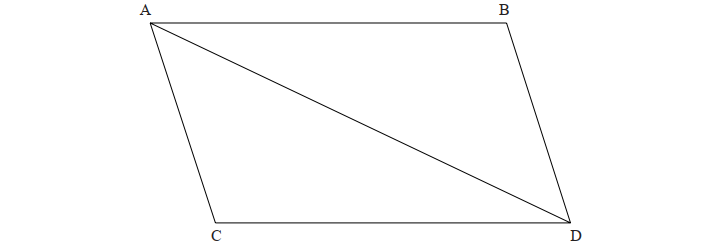
\includegraphics[width=0.75\linewidth]{image/Text3/Fig3.1.png}
\end{figure}
\noindent Let a body in a given time, by force M alone impressed in A, be carried with uniform motion from A to B, and, by force N alone impressed in the same place, be carried from A to C; then complete the parallelogram ABDC, and by both forces the body will be carried in the same time along the diagonal from A to D. For, since force N acts along the line AC parallel to BD, this force, by law 2, will make no change at all in the velocity toward the line BD which is generated by the other force. Therefore, the body will reach the line BD in the same time whether force N is impressed or not, and so at the end of that time will be found somewhere on the line BD. By the same argument, at the end of the same time it will be found somewhere on the line CD, and accordingly it is necessarily found at the intersection D of both lines. And, by law 1, it will go with [uniform] rectilinear motion from A to D.\\
设一个物体在给定时间内,仅在 A 点受到力 M 的作用,以匀速从 A 运动到 B ;并且在同一位置仅受到力 N 的作用,从 A 运动到 C ;然后完成平行四边形 ABDC ,那么在这两个力的共同作用下,物体将在相同时间内沿对角线从 A 运动到 D 。因为力 N 沿着与 BD 平行的直线 AC 起作用,根据第二定律,这个力对由另一个力产生的朝向 BD 线的速度完全不会产生任何改变。因此,无论力 N 是否作用,物体都将在相同时间内到达 BD 线,所以在该时间结束时,物体将出现在 BD 线上的某个位置。通过同样的论证,在相同时间结束时,物体将出现在 CD 线上的某个位置,因此它必然出现在两条线的交点 D 处。并且,根据第一定律,它将从 A 以 [匀速] 直线运动到 D 。\\

\begin{center}
    [...]
\end{center}

\end{document}